\section{CNN}
\label{sec:cnn}

Konvolucijska neuronska mreža (eng. Convolutional neural network, CNN) je vrsta 
umjetne neuronske mreže koja je pogodna je za obradu podataka s rešetkastom
topologijom, a najviše se koristi za rješavanje problema iz područja klasifikacije slika
te računalnog vida. Inspirirane su načinom funkcioniranja moždanog korteksa 
zaduženog za vid kod sisavaca \cite{pycodemates}. Obrada slike koju vide sisavci
funkionira hijerarhijski, tj. u mozgu se ne obrađuje cjelokupna slika odjednom,
nego postoje jednostanije stanice koje su zadužene za prepoznavanje osnovnijih
oblika koji se nakon toga stapaju u složenije i složenije. Na poslijetku 
organizam je u mogućnosti prepoznati cjelokupnu sliku koju gleda očima.

Računalni modeli koji koriste strukturu sličnu opisanoj mogu iz
podataka koji su u takvom obliku izvući značajke samostalno što znači da nema
potrebe za korištenjem metoda koje eksplicitno izvlače bitne značajke iz podataka
\cite{1}. Arhitektura najjednostavnije konvolucijske neuronske mreže
uključuje:

\begin{itemize}
    \item \(Ulaz\) (eng. Input Layer): ulazni sloj modela, prima matrični podatak
    \item \(Konvolucijski\) \(sloj\): osnovni sloj modela. Njegov glavni zadatak
          je ekstrakcija značajki iz ulaznih podataka. Detaljnije je opisan u \ref{sub:conv}.
    \item \(Sloj\) \(za\) \(poduzorkovanje\): smanjuje dimenzionalnost (vidi \ref{sub:pooling})
    \item \(Potpuno\) \(povezani\) \(sloj\): povezuje značajke s klasifikacijom (vidi \ref{sub:dense})
    \item \(Izlaz\) : izlazni sloj, daje vjerojatnosti klasifikacije (vidi \ref{sub:output})
\end{itemize}

\begin{figure}[htb]
    \centering
    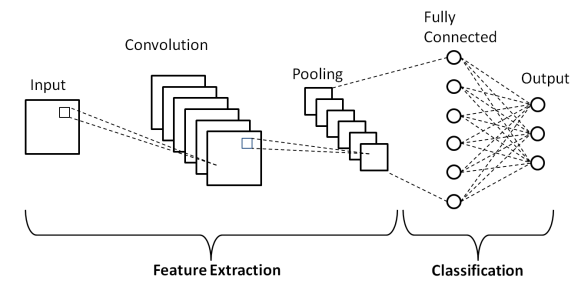
\includegraphics[width=0.5\linewidth]{Chapters/neuronska_mreza/CNN/cnn.png} 
    \caption{Jednostavna CNN \cite{1}}
    \label{pic:cnn}
\end{figure}

Na slici \ref{pic:cnn} prikazana je opisana struktura. Prva tri sloja grupirana su
u dio koji služi za ekstrakciju značajki iz ulaznih podataka, a posljednja dva
sloja služe za klasifikaciju. Složenije arhitekture mreže mogu imati veći broj
konvolucijskih slojeva (nakon svakog se nalazi sloj za poduzorkovanje) te veći broj
složenijih ili manje složenih potpuno povezanih slojeva.

\subsection{Konvolucijski sloj}
\label{sub:conv}

Najbitniji dio konvolucijske neuronske mreže je konvolucijski sloj zbog toga što se
u njemu događa konvolucija. Konvolucija (u neuronskim mrežama) je proces kojim 
iz ulazne matrice podataka (slike) na izlazu dobijemo matricu značajki ili
mapu značajki. Neka ulazna matrica bude oblika \( x \in M_{mn}(\mathbb{R}) \).
Umjesto težina (kao kod potpuno povezanog sloja), konvolucijski sloj koristi
matricu \( \omega \in M_{pr}(\mathbb{R}) \) koju nazivamo filtar ili
jezgra (eng. kernel) \ref{keras_layers}. Svaki konvolucijski 
sloj može imati proizvoljan broj filtara. Izlazna (u ovom slučaju dvodimenzionalna)
mapa značajki tada se računa na sljedeći način:

\begin{equation}
h = \omega * x,
\end{equation}

pri čemu \( * \) označava operaciju konvolucije te vrijedi:

\begin{equation}
h(i, j) = (\omega * x)(i, j) = 
\sum_{k=0}^{p-1} \sum_{l=0}^{r-1} x(i + k, j + l) \omega(k, l).
\end{equation}

Formula koja se zapravo koristi naziva se unakrsna korelacija, međutim, zbog sličnosti s 
formulom konvolucije, mreža nosi takav naziv \ref{gracan2020}. Na slici 
\ref{pic:convolution} prikazan je proces koji se događa tijekom prolaska 
ulaznog podatka kroz konvolucijski sloj. Ulaz (eng. input) se konvolucijski množi
s jezgrom kako bismo dobili izlaznu matricu značajki \cite{cnn_how}. U slučaju prikazanom na slici,
ulazna slika je veličine \(4 \times 4\), dok je jezgra veličine \(3 \times 3\). Prvo se podmatrica ulaznog
podatka veličine jednake veličini jezgre (\(3 \times 3\)) skalarno množi s jezgrom. Izlaz je 
skalarni umnožak na koji se može dodati konstantna vrijednost (eng. bias). Nakon
toga se jezgra pomiče po ulaznoj matrici, tj. sljedeći element izlazne matrice je
skalarni umnožak jezgre i sljedeće podmatrice ulaznog podatka. Koliko će se jezgra
pomaknuti određuje pomak (eng. stride). U slučaju na slici \ref{pic:convolution}
pomak iznosi jedan.

\begin{figure}[htb]
      \centering
      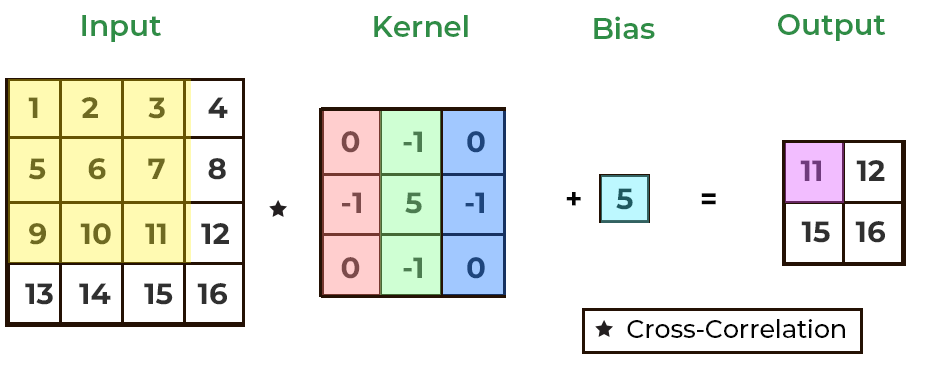
\includegraphics[width=0.5\linewidth]{Chapters/neuronska_mreza/CNN/convolution.png} 
      \caption{Konvolucija \cite{convolution}}
      \label{pic:convolution}
\end{figure}

Rezultat opisanog procesa je mapa značajki koja je manja od ulazne, a njema veličina
obrnuto proporcionalno ovisi o veličini jezgre te pomaku \cite{cnn_whatis}. 

Slično procesu koji se odvija u mozgu čovjeka, opisani struktura omogućava hijerarhijsko učenje.
Naime, svaki konvolucijski sloj sadrži jezgre koje su zadužene za lokalno pretraživanje
određenih uzoraka (upravo konvolucijom izvlačimo stvari koje su slične između različitih
ulaznih slika). Koje jezgre se trebaju koristiti? Vrlo jednostavno, proces učenja (treniranja
mreže) će prepoznati lokalne sličnosti između različitih primjera! Ako strukturiramo mrežu
tako da se sastoji od više uzastopnih konvolucijskih slojeva, mreža će prvo naučiti najjednostavnije
oblike, a zatim u sljedećem sloju takvim oblicima slagati složenije uzorke. Također,
još jedna prednost konvolucijskom sloja je u dijeljenju parametara. Takav sloj nema vezu 
svakog neurona sa svakim ulaznim, nego se težine dijele unutar određene jezgre. Zapravo se
cijeli proces učenja svodi na nalaženje odgovarajućih jezgri koje će prepoznati uzorke \cite{pycodemates}.
Evo uzmimo, na primjer, dvodimenzionalnu ulaznu sliku. Broj pametara takvog dvodimenzionalnog
sloja iznosit će:

\begin{equation}
    N = (n \cdot m \cdot C_{\text{in}} + 1) \cdot C_{\text{out}}
\end{equation}

Gdje:
\begin{itemize}
    \item \(N\): ukupni broj parametara
    \item \(n\) i \(m\): visina i širina filtra (jezgre)
    \item \(C_{\text{in}}\): Broj ulaznih kanala (npr. 1 za crno-bijele slike, 3 za RGB slike).
    \item \(+1\): konstanta svakog filtra
    \item \(C_{\text{out}}\): Broj filtara (odnosno mapa izlaznih značajki).
\end{itemize}

Kako bismo bolje dočarali razliku u broju parametara između ovakog sloja i potpuno povezanog sloja,
uzmimo za primjer sliku \ref{pic:convolution}. Ulazna slika je veličine \(4 \times 4\),
jezgra \(3 \times 3\), a izlaz 
\(2 \times 2\). Neka je slika jednokanalna, a broj jezgri jedan (sve kao na slici). Konvolucijski sloj
će imati 10 parametara, dok će potpuno povezani sloj (16 ulaznih vrijednosti, 4 izlazne te
4 konstante za svaki neuron) imati 68 parametara! Formula za broj parametara u tom slučaju
je sljedeća:

\begin{equation}
    N = n_{\text{in}} \cdot n_{\text{out}} + n_{\text{out}}
\end{equation}

Gdje:
\begin{itemize}
    \item \(N\): ukupni broj parametara
    \item \(n_{\text{in}}\): broj ulaznih neurona
    \item \(n_{\text{out}}\): broj izlaznih neurona
\end{itemize}

Također, kao što je opisano u poglavlju \ref{pog:neuronska_mreza} vrijednost neurona (čvora) na
izlazu it sloja potrebno je provući kroz aktivacijsku funkciju. Postoje različite vrste funkcija
koje se koriste u različitim granama strojnog i dubokog učenja \cite{activation_fcn}, a za
primjenu u konvolucijskim slojevima, najefektivnija se pokazala ReLu (eng. Rectified linear units)
\cite{relu}. To je funkcija koja vraća nulu ako joj je ulaz negativan, a za svaki pozitivan
ulaz samo prosljeđuje istu vrijednost na izlaz. Modelirana je formulama \ref{eq:relu1} i 
\ref{eq:relu2}, a prikazana je na slici \ref{pic:relu}. 

\begin{equation}
    f(x) = \max(0, x)
    \label{eq:relu1}
\end{equation}

\begin{equation}
    f(x) = 
    \begin{cases} 
        0, & \text{ako } x < 0, \\
        x, & \text{ako } x \geq 0.
    \end{cases}
    \label{eq:relu2}
\end{equation}

\begin{figure}[htb]
    \centering
    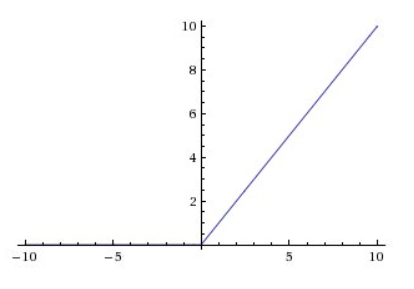
\includegraphics[width=0.5\linewidth]{Chapters/neuronska_mreza/CNN/relu.png} 
    \caption{ReLu \cite{relu}}
    \label{pic:relu}
\end{figure}

Prednosti ReLu funcije nad nad drugim aktivacijskim funkcijama je u tome za negativne
ulaze uopće ne aktivira neuron što izuzetno povećava efikasnost. Druga prednost je u tome
što izlaz nelinearno raste s porastom ulazne vrijednosti što znači da nikad neće ući
u zasićenje. Ta osobina je važna jer utječe na izgled funkcije gubitka te ubrzava
konvergenciju gradijentnog spusta prema minimumu funkcije gubitka \cite{activation_fcn}.


\subsection{Sloj za poduzorkovanje}
\label{sub:pooling}
Sloj za poduzorkvanje (eng. Pooling layer): služi smanjenju dimenzionalnosti matrice
značajki na izlazu iz konvolucijskog sloja. Najčešće korištene tehnike su maksimalno 
(eng. max pooling) i prosječno poduzorkovanje (eng. average pooling). Radi tako da više 
susjednih vrijednosti spoji u jednu te tako na svom izlazu da matricu manjih dimenzija 
\cite{pooling1}. Na taj način postupno smanjuje broj parametara, smanjuje broj
operacija potrebnih za daljnje računanje te ono najbitnije, kontrolira
prenaučenost \cite{cnn_whatis}. Na slici \ref{pic:pooling} prikazane su obje navedene vrste poduzorkovanja.

\begin{figure}[htb]
    \centering
    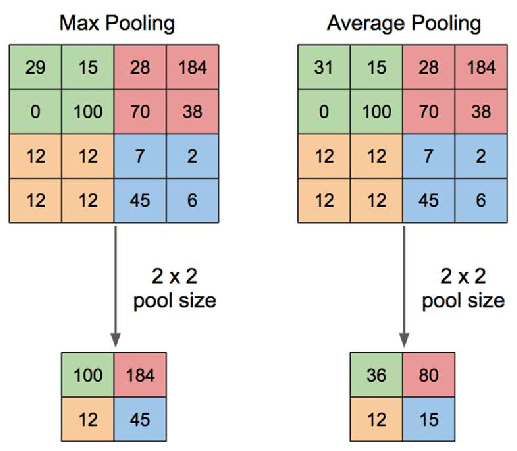
\includegraphics[width=0.5\linewidth]{Chapters/neuronska_mreza/CNN/pooling.png} 
    \caption{Poduzorkovanje \cite{pooling1}}
    \label{pic:pooling}
\end{figure}

Prosječno poduzorkovanje izglađuje sliku (eng. smoothing). Zbog toga oštri detalji slike
mogu biti izgubljeni što znači da se određene značajke možda neće prepoznati kada se 
koristi ova metoda. Maksimalno uzorkovanje odabire najsvjetlije piksele iz slike,
a oni su se pokazali kao najbitnije značajke jer daju najbolje rezultate \cite{cnn_whatis}.
Suprotno tome, minimalno uzorkovanje (eng. min pooling) odabralo bi najtamnije piksele,
međutim ono se najrjeđe koristi.

\subsection{Sloj za poravnavanje}
Sloj za poravnavanje (eng. flatten layer) je sloj koji dolazi nakon posjednjeg sloja
za poduzorkovanje. Njegova jedina zadaća je poravnati izlaz iz prijašnjeg sloja.
Ovaj sloj ništa ne računa, ništa ne uči, jedina zadaća mu je od ulaznih mapa značajki
napraviti jedan vektor koji je onda moguće povezati na potpuno povezani sloj. Zbog
toga se često izostavi iz skica koje prikazuju strukture CNN-ova kao što je slučaj
na slici \ref{pic:cnn}. Na slici \ref{pic:flatten} prikazana je uloga ovog sloja.

\begin{figure}[htb]
    \centering
    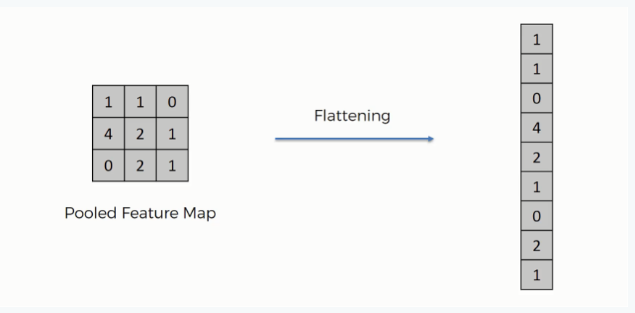
\includegraphics[width=0.5\linewidth]{Chapters/neuronska_mreza/CNN/flatten.png} 
    \caption{Sloj za poravnjavanje \cite{flatten}}
    \label{pic:flatten}
\end{figure}


\subsection{Potpuno povezani sloj}
\label{sub:dense}
Potpuno povezani sloj (eng. Fully Connected Layer) detaljnije je pojašnjen u poglavlju
\ref{pog:neuronska_mreza}. Nakon prijašnjih slojeva koji su služili za izvlačenje
značajki iz ulaznih podataka, na red dolazi klasifikacija. Budući da je prethodnik
prvom ovakvom sloju sloj za poravnavanje, nemamo problem sa spajanje ovog sloja na dosad
objašnjenu strukturu. Uloga ovog sloja (ili više ovakvih slojeva) je, najjednostavnije
rečeno, klasifikacija. Značajke naučene tijekom konvolucije se ovdje predaju gustoj mreži
neurona koja je sposobna odraditi posao do kraja, tj. naučiti kako različite značajke
pridonose određenoj izlaznoj klasi.

\subsection{Izlazni sloj}
\label{sub:output}
Izlazni (eng. Output Layer) je posljednji sloj potpuno povezanog sloja (a ujedno i cijele
neuronske mreže). Ima onoliko neurona koliko želimo imati klasa, pojedina vrijednost
neurona predstavlja vjerojatnost pripadnosti klasi. Da bi to stvarno funkcioniralo na takav
način, potrebno je odrediti prikladnu aktivacijsku funkciju. Funkcija koja radi baš to 
naziva se funkcija softmax. 
Formalno, \( \text{softmax} : \mathbb{R}^n \to \mathbb{R}^n \),
gdje je \( k \)-ta komponenta izlaznog vektora definirana kao:
\begin{equation}
\text{softmax}_k(x_1, \dots, x_n) = \frac{\exp(x_k)}{\sum_{j} \exp(x_j)}
\end{equation}

Funkcija softmax radi dvije ključne stvari:
\begin{itemize}
    \item Normalizira sve vrijednosti tako da njihov zbroj bude \( 1 \), tj. izlazni vektor 
        predstavlja distribuciju vjerojatnosti.
    \item Pojačava veće vrijednosti (čini ih dominantnijima) i smanjuje manje vrijednosti.
\end{itemize}

Funkcija nosi naziv \textit{softmax} jer odgovara funkciji \( \max \), ali je "meka" u smislu
da je neprekidna i diferencijabilna, za razliku od klasične \( \max \) funkcije 
\cite{snajder2023logreg}.

\begin{figure}[htb]
    \centering
    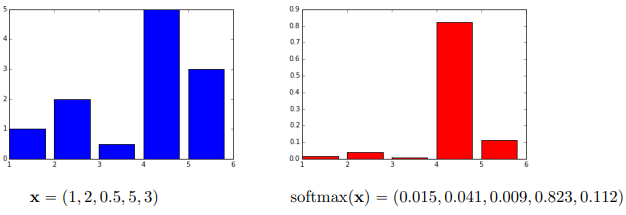
\includegraphics[width=0.6\linewidth]{Chapters/neuronska_mreza/CNN/softmax.png} 
    \caption{Softmax \cite{snajder2023logreg}}
    \label{pic:softmax}
\end{figure}


\subsection{Poznate arhitekture konvolucijskih mreža}
Arhitektura konvolucijske mreže je ključni faktor koji određuje njene performanse i
učinkovitost. Broj konvolucijskih slojeva, izgled istih (broj filtara, njihova veličina,
pomak), vrsta slojeva za poduzorkovanje te broj i veličina potpuno povezanih slojeva znatno
utječu na brzinu izvođenja i preciznost klasifikacije. Naravno, ne postoji jedan recept koji
najbolje radi na svim vrstama ulaznih podataka, nego različite arhitekture daju bolje rezultate
u određenim situacijama. Određene arhitekture su kroz povijest ostale zapamćene zbog
toga kako su utjecale na duboko učenje\cite{indian}:

\begin{itemize}
    \item \textbf{LeNet-5 (1998):} 
    CNN sa 7 slojeva dizajnirana za klasifikaciju rukom pisanih brojeva na slikama 
    veličine \(32 \times 32\) piksela u sivim tonovima. Koristila se u bankama za čitanje čekova 
    i bila je prvi značajan korak u korištenju CNN-a u stvarnom svijetu.

    \item \textbf{AlexNet (2012):} 
    Proširena verzija LeNet-a s dubljom arhitekturom (5 konvolucijskih i 3 potpuno povezana 
    sloja). Prva mreža koja je koristila ReLU aktivaciju za brže treniranje. Značajno smanjila
    stopu pogreške na ILSVRC natjecanju i popularizirala duboko učenje.

    \item \textbf{GoogleNet (Inception V1) (2014):} 
    22-slojna mreža s inovativnim \emph{inception module}, koji koristi male konvolucije za 
    smanjenje broja parametara (sa 60 milijuna na samo 4 milijuna). Pobjednik ILSVRC 2014 s 
    top-5 pogreškom manjom od 7\%. Performanse su usporedive s ljudskim prepoznavanjem slika.

    \item \textbf{VGGNet (2014):} 
    Mreža sa 16 konvolucijskih slojeva koja koristi samo \(3 \times 3\) konvolucije s povećanim
    brojem filtara. Iako je jednostavna u dizajnu, ima 138 milijuna parametara, što je čini 
    računalno zahtjevnom za treniranje i implementaciju.
\end{itemize}